\section{The signal: dijet resonance}
\label{sec:signal}

We search for dijet resonances corresponding to several models.
Using the W/Z-tagging algorithm, we examine both single W/Z-tag and double W/Z-tag events.

The pruned jet mass and jet $\tau_{21}$ distributions in signal MC, data and background MC are shown in Figure~\ref{fig:taggingvariables}.
Fully merged jets from hadronic W and Z decays peak around 80$\sim$90\GeVcc while QCD jets and not fully merged W and Z jets peak around 20 GeV.
The distribution
of $\tau_{21}$ for ${\rm W/Z \to qq\prime}$ signal, peaks around 0.4 and is almost
fully contained within $\tau_{21} < 0.75$, where we place our cut; 
in contrast, QCD background peaks ${\sim}0.7-0.8$. 
The discriminating power of the pruned jet mass and $\tau_{21}$ is evident.


The modelling of the signal efficiency is cross-checked through a W-tagging efficiency 
estimated using merged ${\rm W \to qq\prime}$ decays in $\ttbar$
events~\cite{JME-13-006}. The efficiency is obtained using ${\rm \ell + jets}$ events with two b-tagged jets, 
one of which has $\pt > 200$~GeV. Such events are dominated by $\ttbar$
production. The data are compared to simulated $\ttbar$ events, 
generated with MADGRAPH, interfaced to 
\PYTHIA~for parton showering, and provide scale factors of 
$0.86 \pm 0.07$ and $1.39 \pm 0.75$,
respectively, for HP and LP events. 
These values are derived following the method described in Ref~\cite{JME-13-006}
 for the selections applied in this analysis, and are used to match the 
 simulated samples to data. 
 The uncertainties in the scale factors contribute to the systematic uncertainty in 
 the selection efficiency for signal.


For both the pruned jet mass and $\tau_{21}$, differences are observed
between the \HERWIG{++} ($G_{RS}$) and \PYTHIA~6
($G_{Bulk}$, $\cPq^*$, $\PWpr$) distributions, which arise from
differences in the polarization of the $\PW$/$\cPZ$ boson and the
showering and hadronization models used by these generators. 
%In
%particular this is the reason why the $\PW\cPZ$ prediction for
%$\tau_{21}$ is different from the $\PW\PW$, $\cPZ\cPZ$ predictions.
The differences, due to showering and hadronization,
are taken into account in estimating the systematic uncertainties
on the tagging efficiencies, as discussed below.

\begin{figure}[htb]
\begin{center}
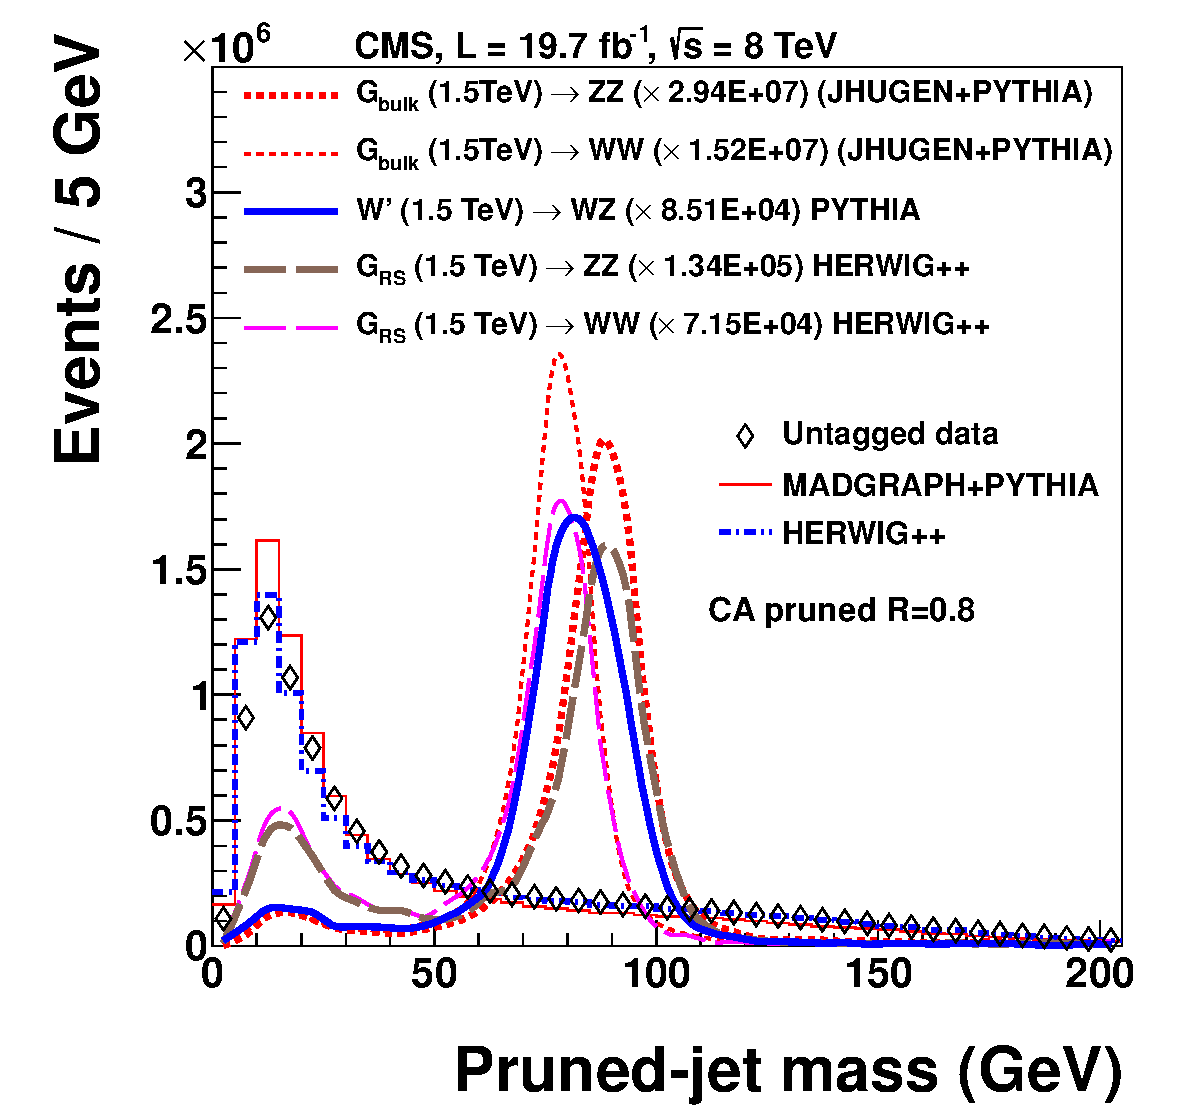
\includegraphics[width=0.49\textwidth]{EXO-12-024/figs/signal-acc-eff/signal-data-qcd-jetmass.pdf}
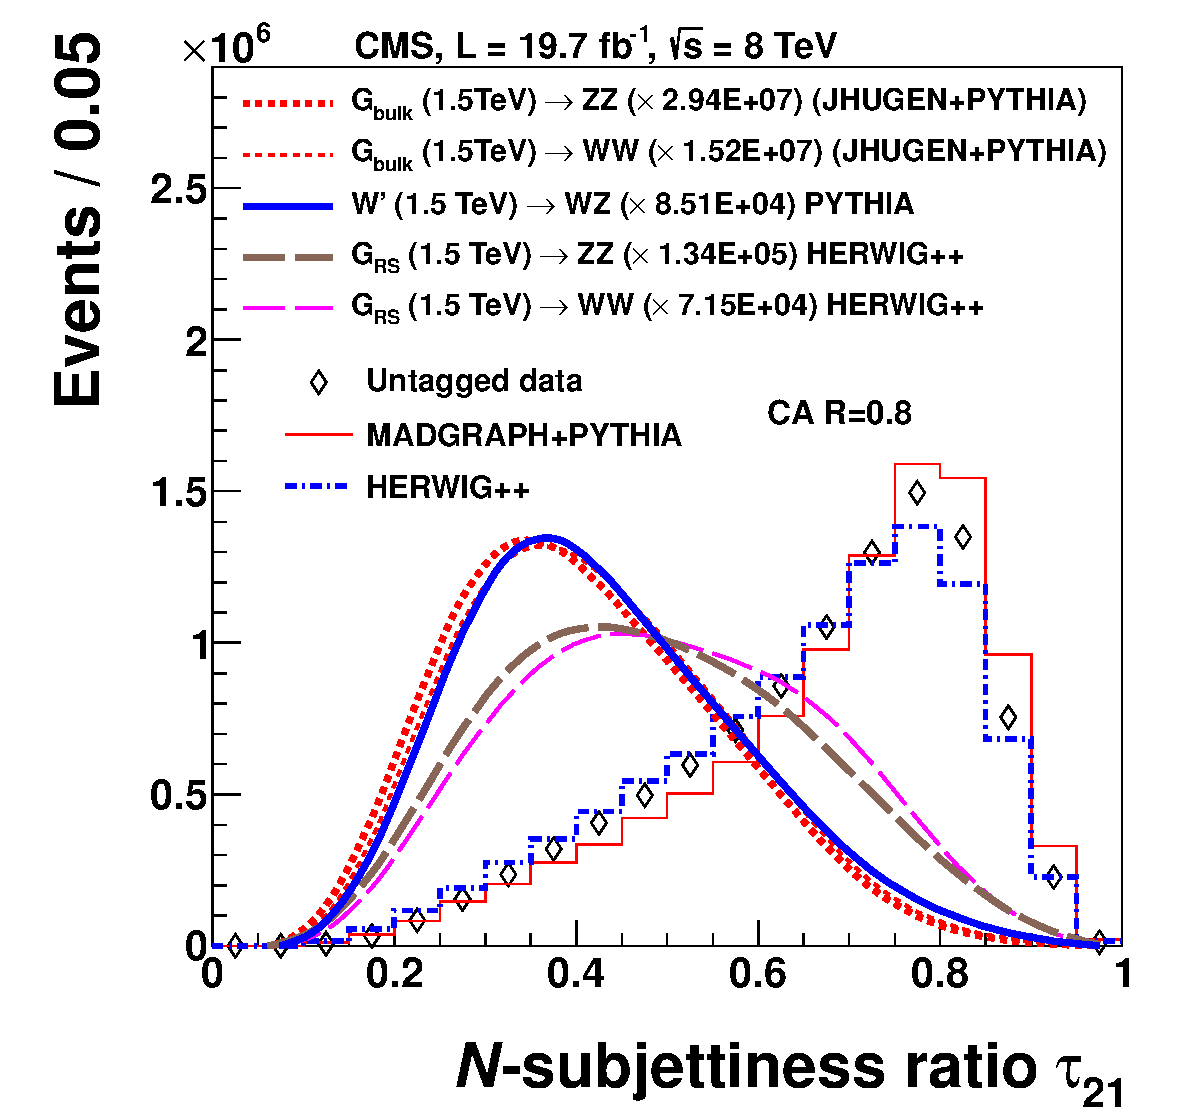
\includegraphics[width=0.49\textwidth]{EXO-12-024/figs/signal-acc-eff/signal-data-qcd-Jet-Tau21.pdf}
\end{center}
\caption{
Distribution for (left) pruned-jet mass ${\rm m_j}$ and (right) jet N-subjettiness ratio $\tau_{21}$ 
in data, and in simulations of signal and background events.
 All simulated distributions are scaled to match the number of events in data. 
 MADGRAPH/\PYTHIA and \HERWIG{++} refer to QCD multijet event simulations. 
}
\label{fig:taggingvariables}
\end{figure}

%Table~\ref{table:acceptance} summarizes the signal branching ratio times angular acceptances and also the W/Z-tagging efficiencies.

The full event selection efficiency is estimated using simulated
signal samples.
Less than 1\% of the $\cPZ\cPZ$ or $\PW\PW$ events which pass the full
selection are from $\cPZ\cPZ \to ll qq$ or $\PW\PW \to l\nu qq$
decays, where $l$ can be a muon or electron.  While 3\% of the
selected $\cPZ\cPZ$ events are from $\cPZ\cPZ \to \tau\tau qq$ decays,
less than 1\% of the selected $\PW\PW$ events are from $\PW\PW \to
\tau\nu qq$ decays.
To within 10\% accuracy,  the full selection efficiency can
therefore be
approximated by the product of the $\PW/\cPZ$-tagging efficiency
and an approximate acceptance.
This acceptance is shown in Figure~\ref{fig:acceptances} and
takes into account the angular acceptance
($|\eta| < 2.5$, $|\Delta\eta|<1.3$),
the branching faction into quark final states
$\mathcal{B}$(${\rm \PW/\cPZ \to qq\prime}$),  and a matching within
$\Delta R = \sqrt{(\Delta \eta)^2 + (\Delta\phi)^2} <0.5$
between the generated W/Z bosons and the reconstructed jets.



%\begin{table}[htb]
%\begin{center}
%\begin{tabular}{ |c|c|c|c|c|c| }
%\hline
%signal & model & mass & BR($W/Z \to jets$)$\times$acc. & 1 W/Z-tag & 2 W/Z-tag\\
%\hline
%hline
%\end{tabular} 
%\end{center}
%\caption{Summary of signal branching ratio times acceptance and W/Z-tagging efficiency.}
%\label{table:acceptance}
%\end{table}

\begin{figure}[htb]
\begin{center}
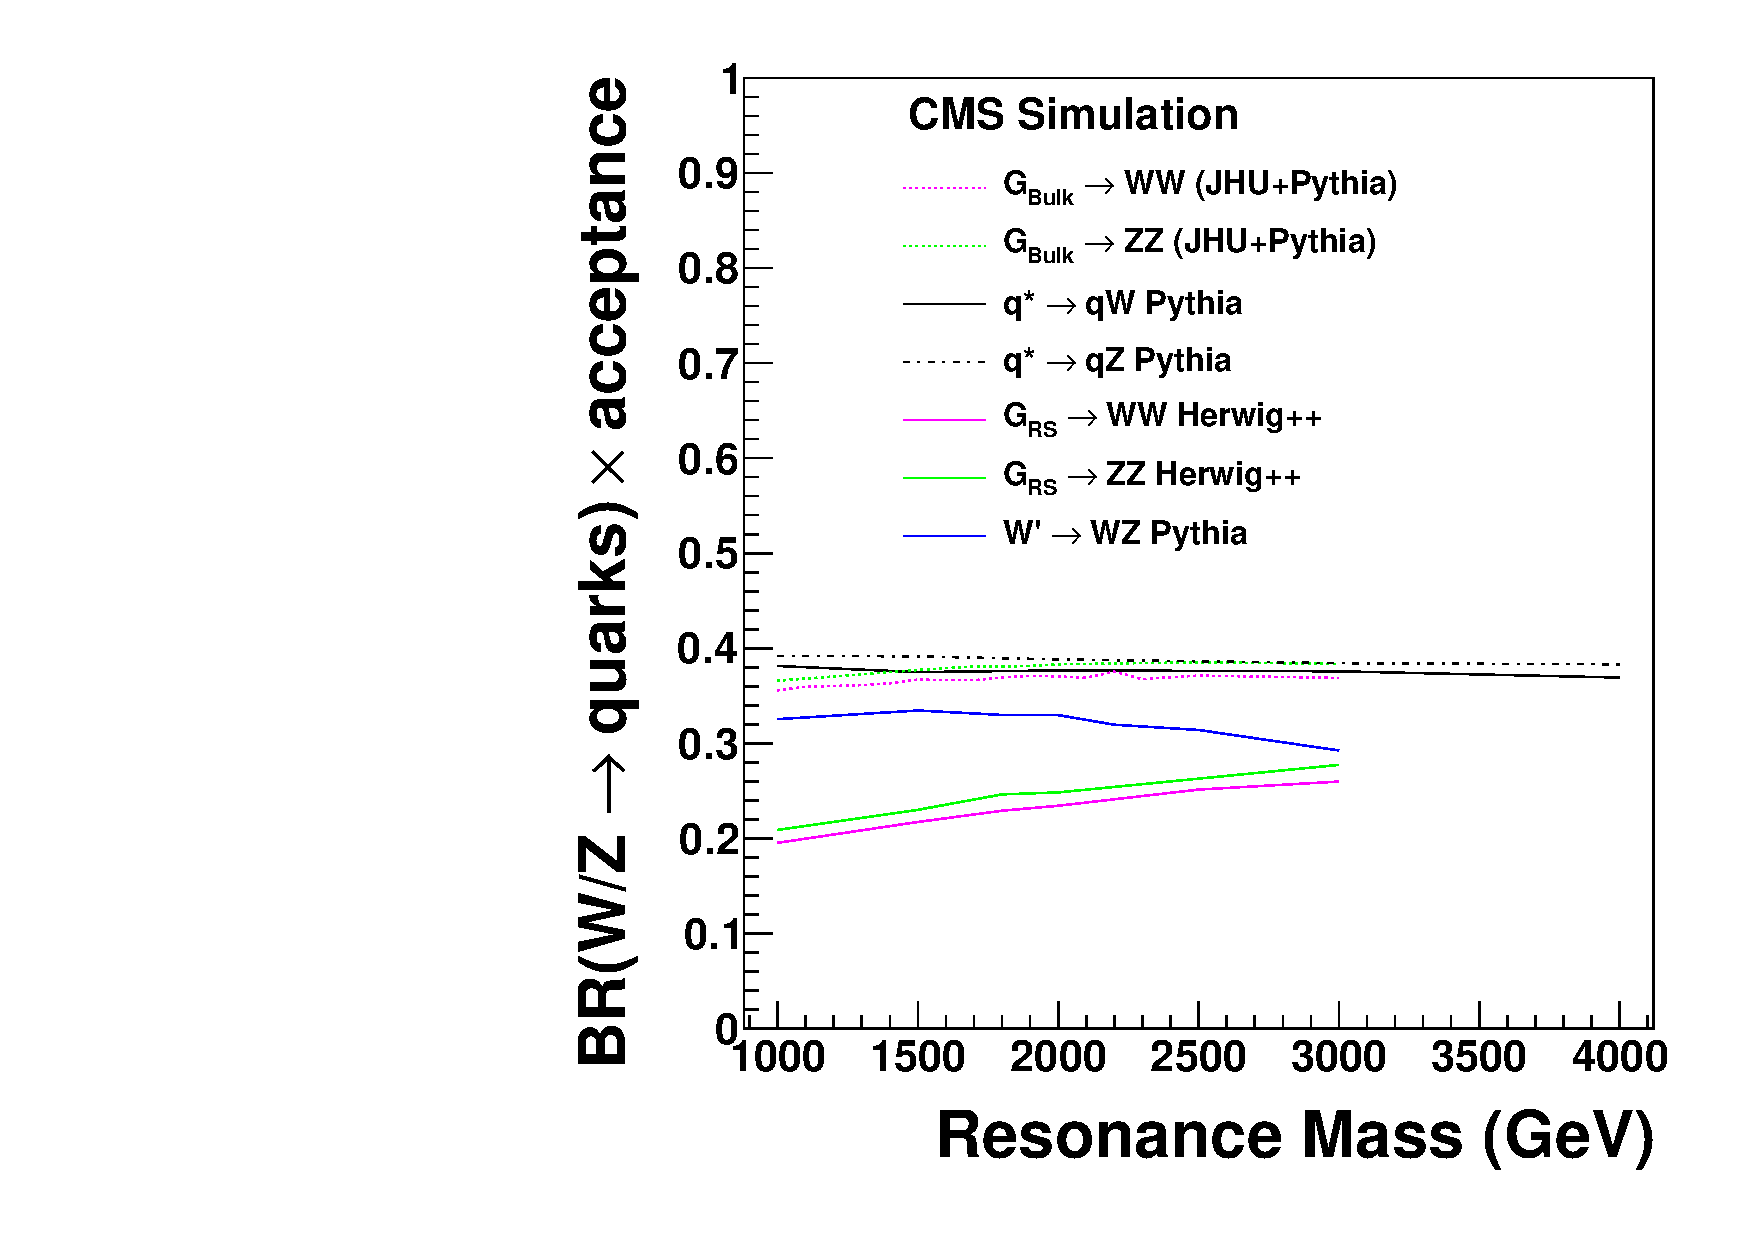
\includegraphics[width=0.6\textwidth]{EXO-12-024/figs/signal-acc-eff/all-signal-acc-8TeV.pdf}
\end{center}
\caption{
The fraction of simulated signal events expected for vector bosons decaying into two quarks,
reconstructed as two jets, that pass the geometrical acceptance criteria ($|\eta| < 2.5$, $|\Delta\eta|<1.3$), shown as a function of the dijet invariant mass.  }
\label{fig:acceptances}
\end{figure}


\begin{figure}[th!b]
\centering
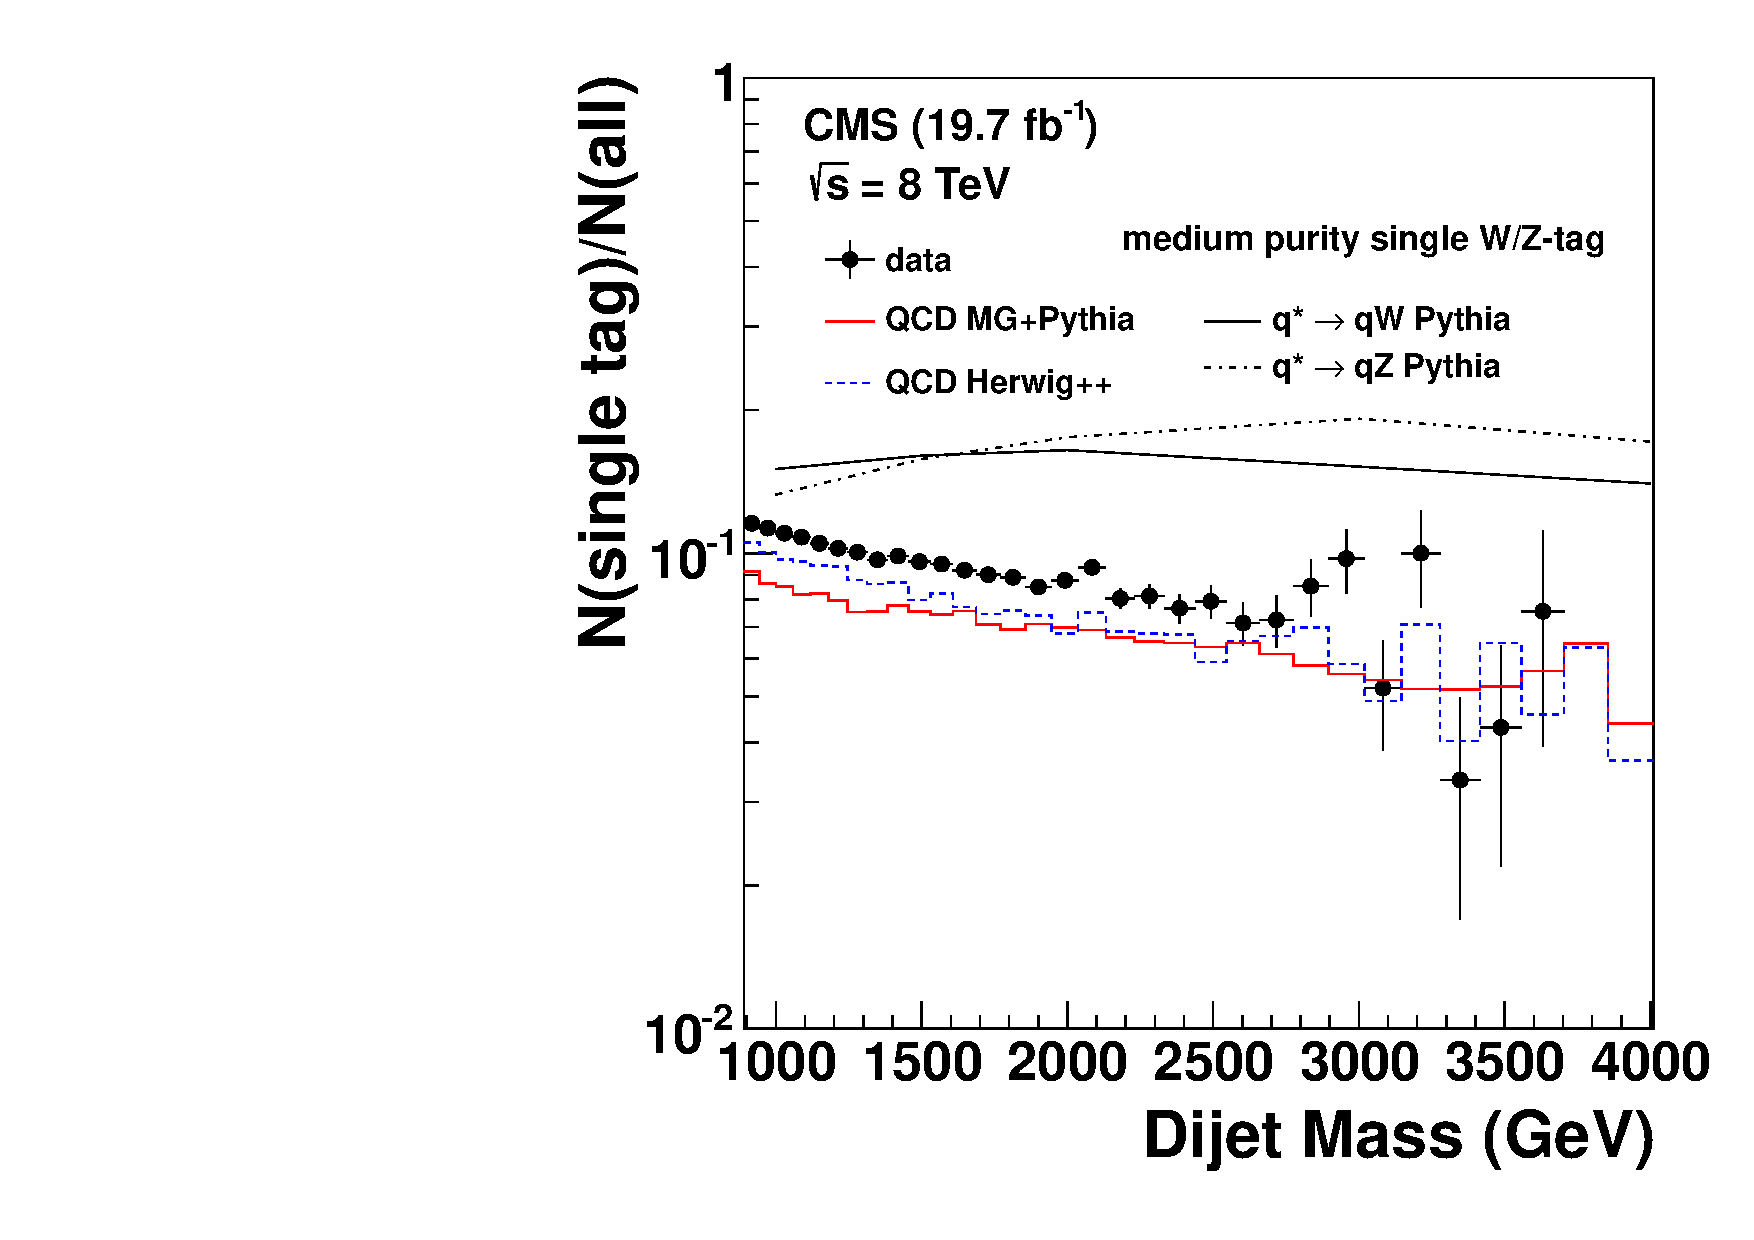
\includegraphics[width=0.49\textwidth]{EXO-12-024/figs/signal-acc-eff/single-tagging-eff-medium.pdf}
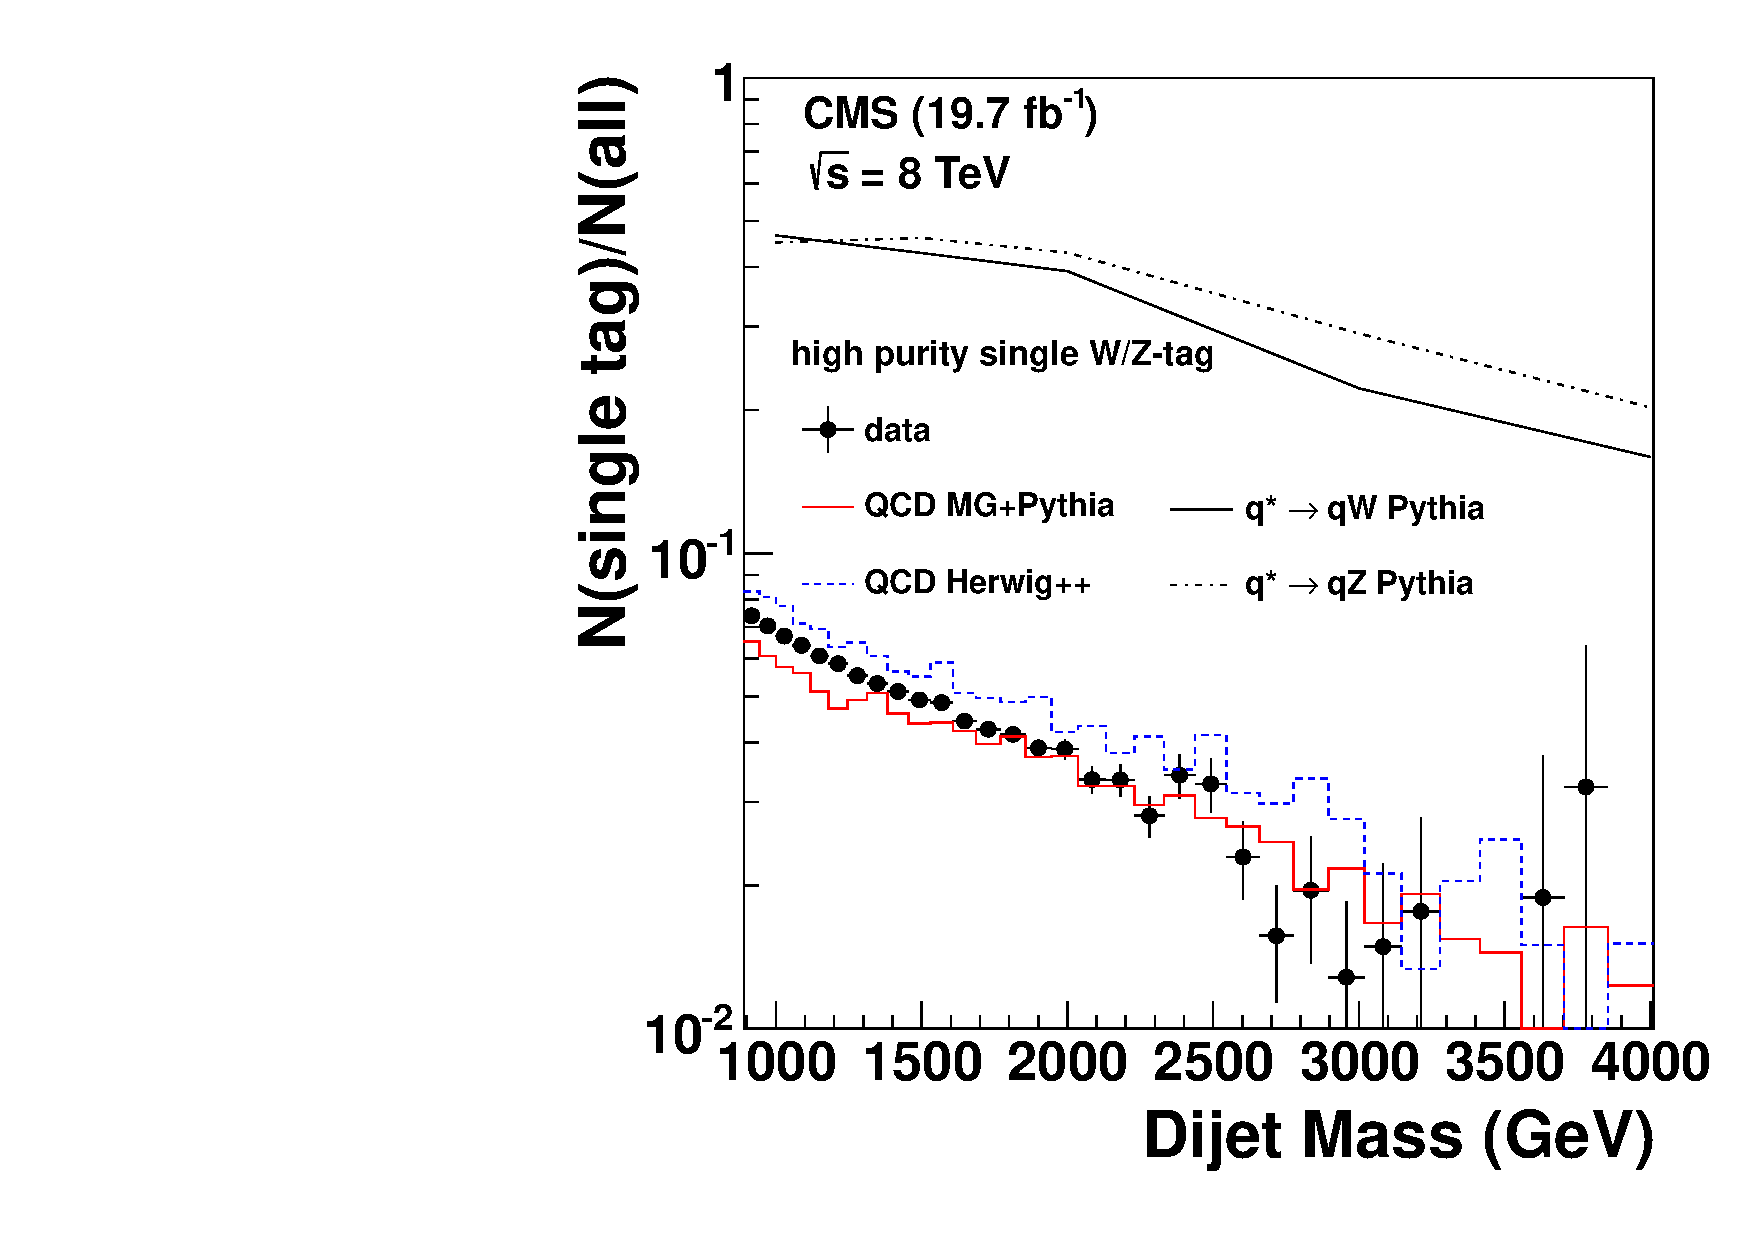
\includegraphics[width=0.49\textwidth]{EXO-12-024/figs/signal-acc-eff/single-tagging-eff.pdf}
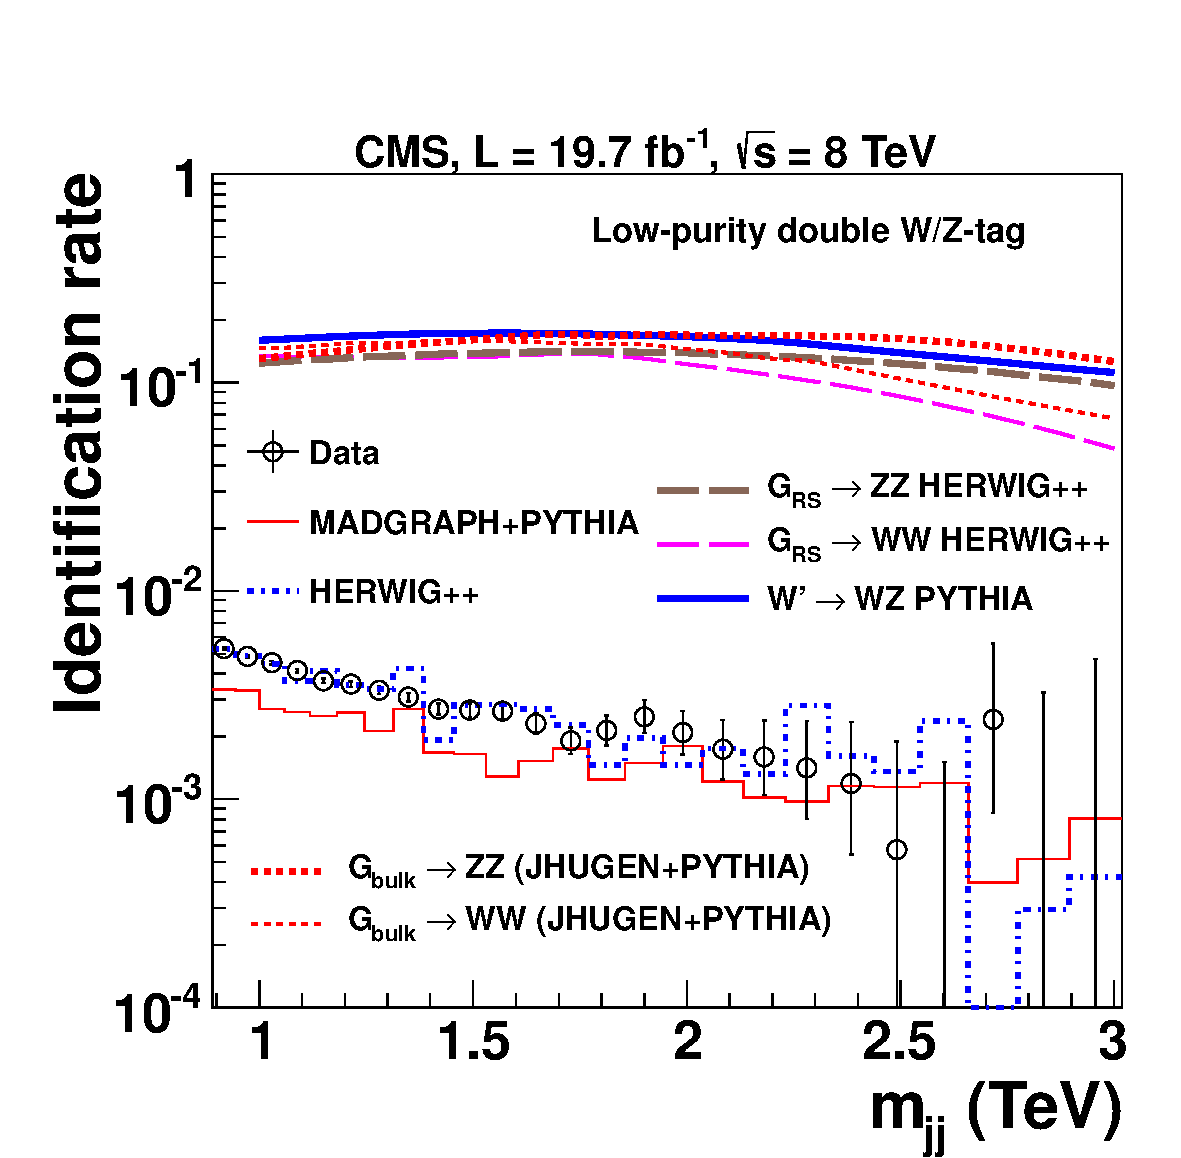
\includegraphics[width=0.49\textwidth]{EXO-12-024/figs/signal-acc-eff/double-tagging-eff-medium.pdf}
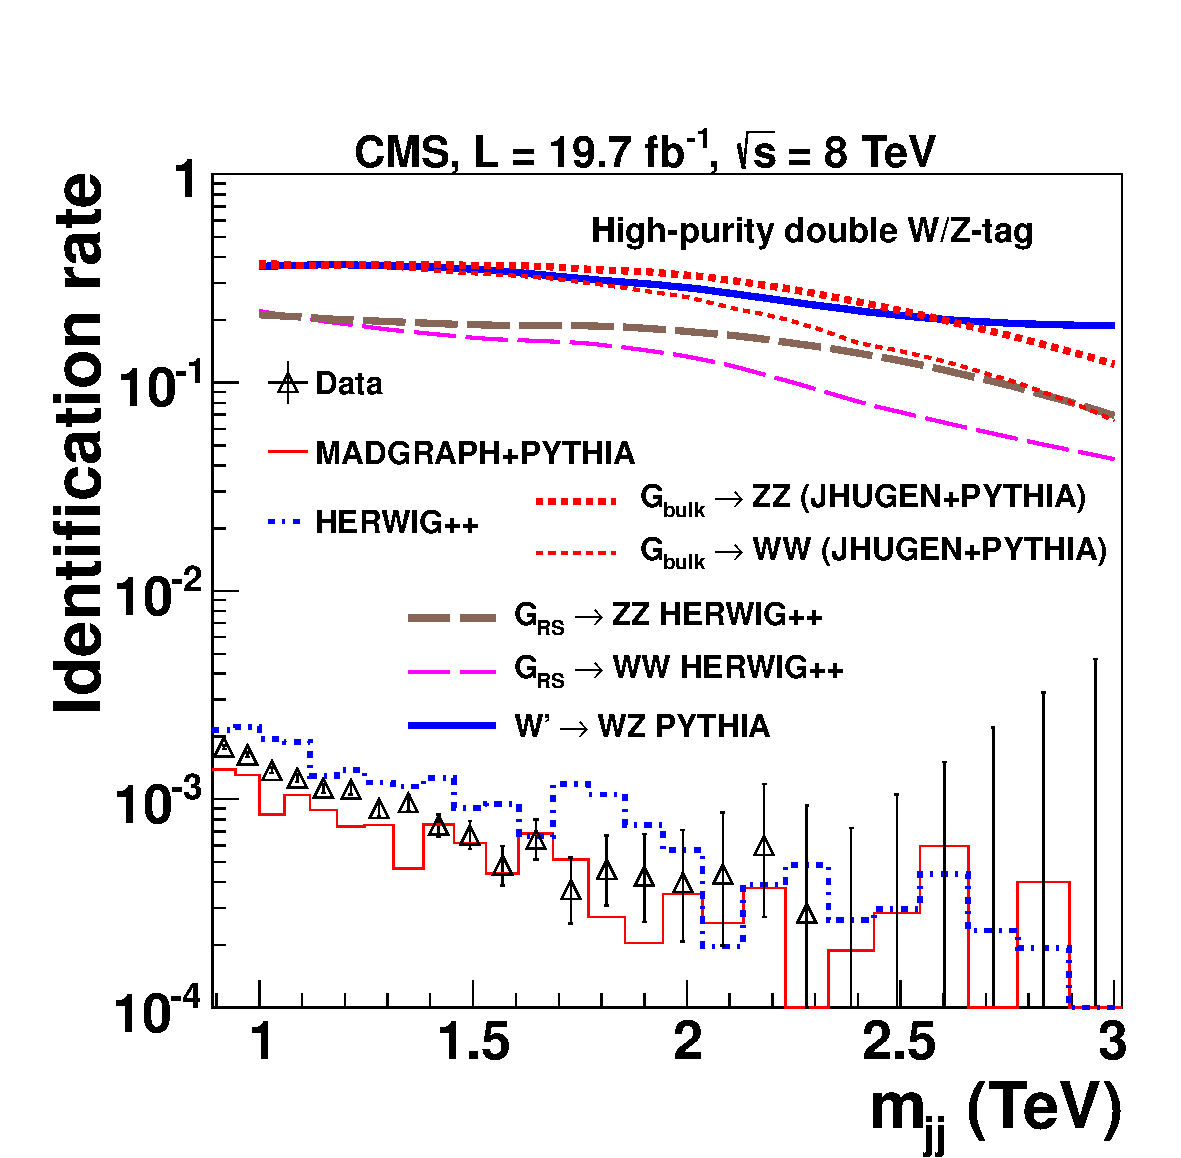
\includegraphics[width=0.49\textwidth]{EXO-12-024/figs/signal-acc-eff/double-tagging-eff.pdf}

\caption{Identification rate for \PW\ and \cPZ\ boson selections
  as a function of $m_\mathrm{jj}$ for quark and gluon
  jets in data and in simulation of background events,
  and for jets from \PW\ and \cPZ\ bosons in simulation of signal events,
  with (upper left) one LP or (upper
  right) HP $\PW/\cPZ$-tag, and the fraction of (lower left)
  doubly-tagged events in the LP and (lower right) HP category. The
  identification rate is computed for $\PW/\cPZ\to q\bar q' \to \text{jets}$
  events, where the jets have $|\eta| < 2.5$ and
  $| \Delta\eta |<1.3$.  \MADGRAPH/\PYTHIA and \HERWIG{++} refer to
  QCD multijet event simulations.
  \label{fig:WZefficiencies}}
\end{figure}



The W/Z-tagging efficiency and also the tag rate in data are shown in 
Figure~\ref{fig:WZefficiencies}. Since data is dominated by background events, the tag rate
in data could be viewed as mistag rate. 


The signal shapes of the HP category for all the processes considered in this analysis are shown in 
Figure~\ref{fig:highsignalShapes}.  
For the qW and qZ final states, the signal shapes with a single W/Z-tag required are shown, while for the other signals two W/Z-tags are required.


%Fig~\ref{fig:acceptanceGstarWWherwig} and Fig~\ref{fig:acceptanceGstarWWpythia} show the signal shape for process: $G_{RS} \to WW$.
%Fig~\ref{fig:acceptanceGstarZZherwig} and Fig~\ref{fig:acceptanceGstarZZpythia} show the signal shape for process: $G_{RS} \to ZZ$.  
%Fig~\ref{fig:acceptanceWprime} shows the signal shape for process: $W' \to WZ$. 
%Fig~\ref{fig:acceptanceqstarqW} and Fig~\ref{fig:acceptanceqstarqZ} shows the signal shape for process: $q* \to qW$, $qZ$.
%The different line colors correspond to different signal resonance masses.
%The dashed line is for signal with a single W/Z-tag, while the dotted 
%line is for signal with two W/Z-tags.

\begin{figure}[htb]
\begin{center}
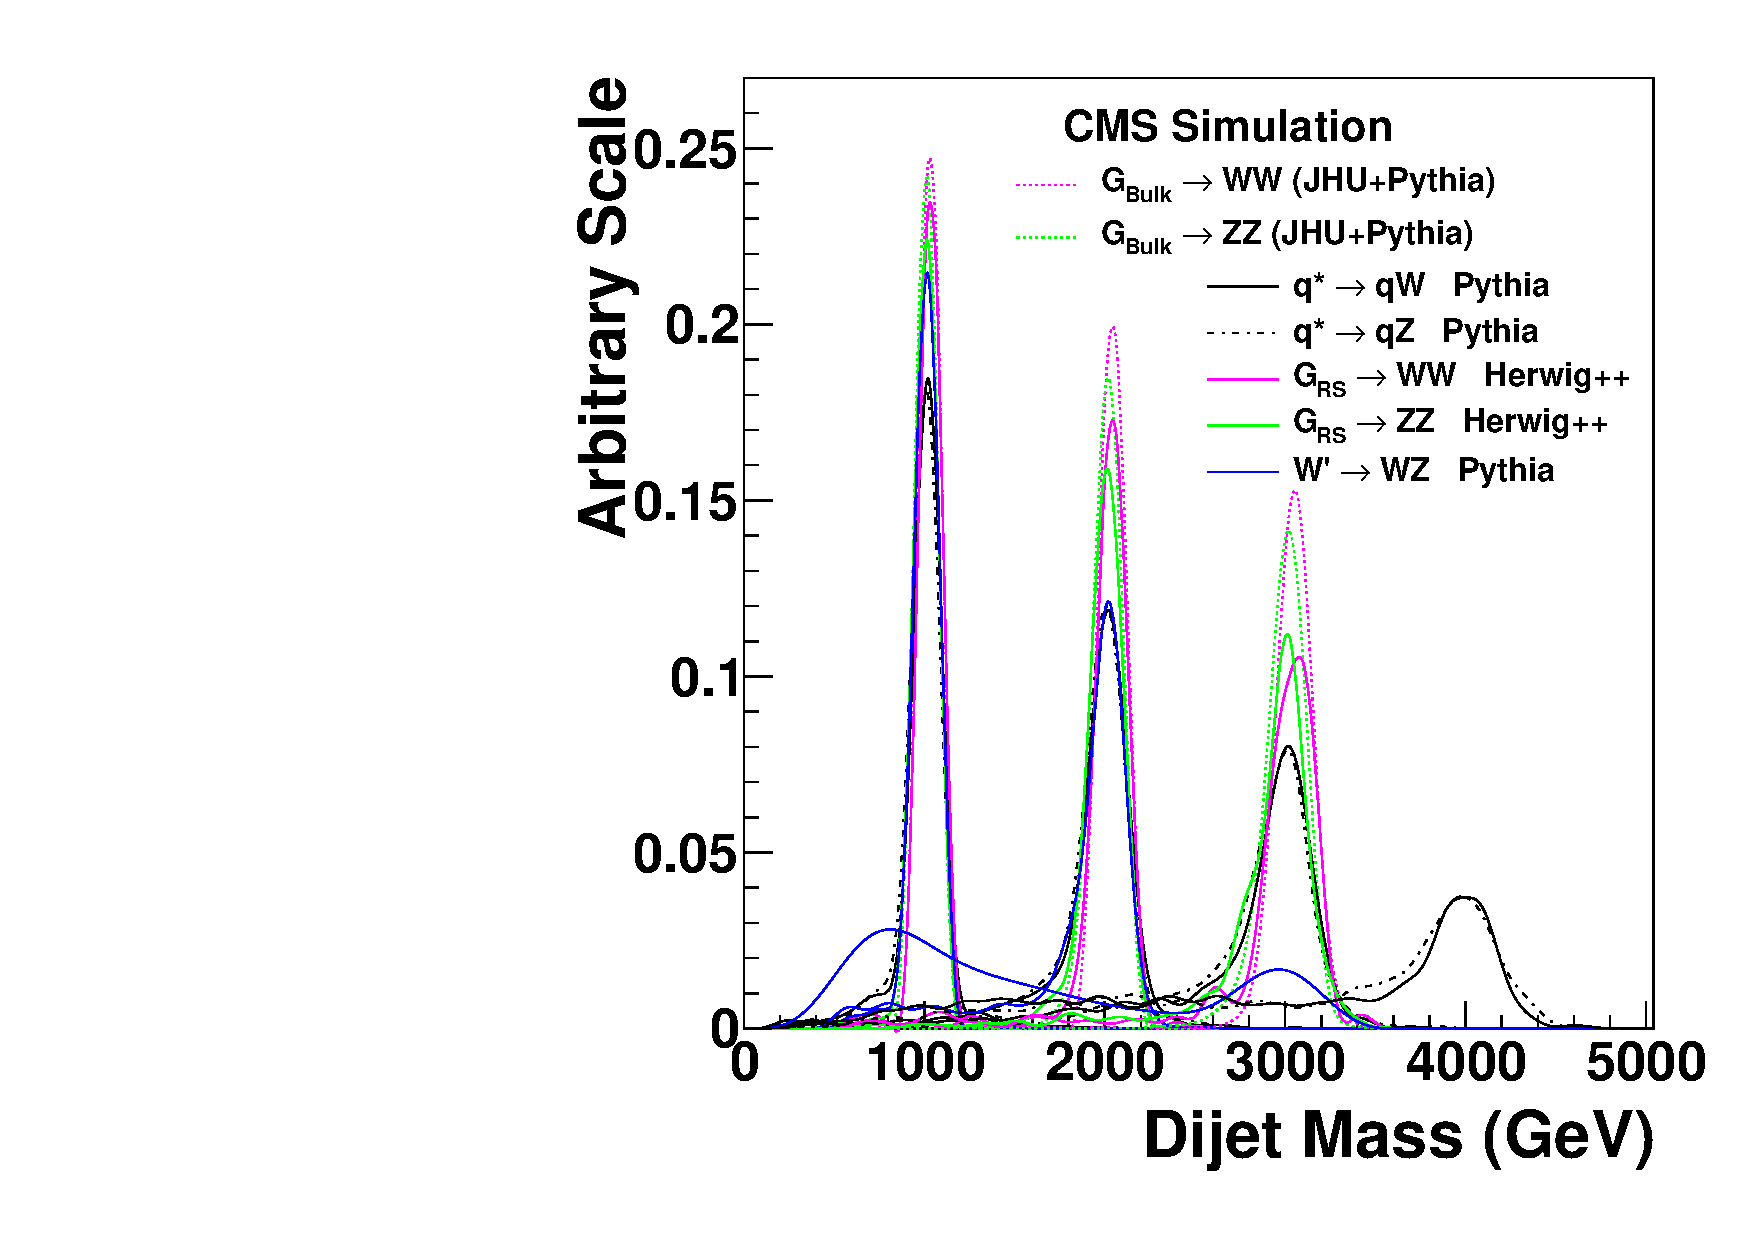
\includegraphics[width=0.6\textwidth]{EXO-12-024/figs/signal-acc-eff/resonance-shape.pdf}
\end{center}
\caption{The normalized HP signal resonance distribution for  $G_{RS}\to WW$, $G_{RS}\to ZZ$, $W' \to WZ$, $q*\to qW$, and $q*\to qZ$ resonances of dijet invariant mass 1.0\TeVcc, 1.5\TeVcc, 2.0\TeVcc,  3.0\TeVcc, 4.0\TeVcc.
}
\label{fig:highsignalShapes}
\end{figure}



\clearpage

